\NeedsTeXFormat{LaTeX2e}
\documentclass[11pt]{article}
\usepackage{url}
\usepackage{amsmath}
\usepackage{amsthm}
\usepackage{amssymb}
\usepackage{mathpartir}
\usepackage{graphicx}
\usepackage{comment}


\newcommand{\deftech}[1]{\textbf{#1}}
\newcommand\mrel{\mathop{\mathbf{r}}}
\newcommand\morel{\mathop{\mathbf{r}'}}
\newcommand\menv{\rho}
\newcommand\mval{v}
\newcommand\mans{a}
\newcommand\mint{i}
\newcommand\moint{j}
\newcommand\mbool{b}

\newcommand\plug[2]{#1[#2]}

\newcommand\merr{r}

\newcommand\mctx{\mathcal{C}}
\newcommand\mectx{\mathcal{E}}
\newtheorem{theorem}{Theorem}
\newcommand\Err{\mathit{Err}}
\newcommand\Plus{\mathit{Plus}}
\newcommand\Mult{\mathit{Mult}}
\newcommand\Succ{\mathit{Succ}}
\newcommand\Pred{\mathit{Pred}}
\newcommand\Eq{\mathit{Eq}}
\newcommand\True{\mathit{True}}
\newcommand\False{\mathit{False}}
\newcommand\If{\mathit{If}}
\newcommand\Div{\mathit{Div}}

\newcommand\reduce{\mathop{\mathbf{b}}}

\newcommand\areducename{\mathbf{a}}
\newcommand\areduce[2]{#1\;\areducename\;#2}

\newcommand\step{\rightarrow_\mathbf{b}}
\newcommand\multistep{\rightarrow^\star_\mathbf{b}}

\newcommand\astdstep{\longmapsto_{\reduce}}
\newcommand\astdmultistep{\longmapsto^\star_{\reduce}}

\newcommand\breducename{\mathbf{b}}
\newcommand\errreducename{\mathbf{err}}
\newcommand\propreducename{\mathbf{prop}}
\newcommand\bvreducename{\mathbf{bv}}
\newcommand\bstepname{\rightarrow_{\breducename}}
\newcommand\bmultistepname{\rightarrow^\star_{\breducename}}

\newcommand\bmultistep[3]{#1\vdash #2\;\bmultistepname\;#3}
\newcommand\bstdstep[3]{#1\vdash #2\;{\longmapsto_{\breducename}}\;#3}
\newcommand\bstdmultistep[3]{#1\vdash #2\;{\longmapsto^\star_{\breducename}}\;#3}

\newcommand\breduce[3]{#1 \vdash {#2}\;\breducename\; {#3}}
\newcommand\errreduce[3]{#1 \vdash {#2}\;\errreducename\; {#3}}
\newcommand\propreduce[3]{#1 \vdash {#2}\;\propreducename\; {#3}}
\newcommand\bvreduce[3]{#1 \vdash {#2}\;\bvreducename\; {#3}}
\newcommand\bstep[3]{#1 \vdash {#2}\;\rightarrow_{\breducename}\; {#3}}
\newcommand\bclosedstep[2]{{#1}\;\rightarrow_{\breducename}\; {#2}}

\newcommand\laxparstep{\rightrightarrows_\mathbf{a}}
\newcommand\maxparstep{\rightrightarrows'_\mathbf{a}}


\newcommand{\xdown}[1]{X_{#1 \downarrow}}
\newcommand{\xup}[1]{X_{#1 \uparrow}}
\newcommand{\xdownk}[2]{X_{#1 \downarrow #2}}
\newcommand{\xupk}[2]{X_{#1 \uparrow #2}}
\newcommand{\xblock}[1]{[x_{#1 1}, x_{#1 2} , \dots, x_{#1 \frac{1}{c}}]^{\top}}
\newcommand{\conpr}[2]{Pr[#1\,|\,#2]}
\newcommand{\priv}{{\bf priv}(X)}
\newcommand{\alt}[1]{{\bf alt}(X_{#1})}
\newcommand{\xbot}[1]{x_{#1 \frac{1}{c}}}
\newcommand{\cwp}[1]{(\epsilon, \delta, \Delta_{#1}, \Gamma)}


\newcommand\Arith{\mathcal{A}}
\newcommand\Barith{\mathcal{B}}

\newcommand\Var{\mathit{Var}}

\newcommand{\mvar}{x}
\newcommand\s[1]{\mathit{#1}}

\title{Streaming CW-Pivacy}
\date{\today}
\begin{document}
\maketitle
\section{Streaming Setting 1}
\begin{figure}[th]
\centering
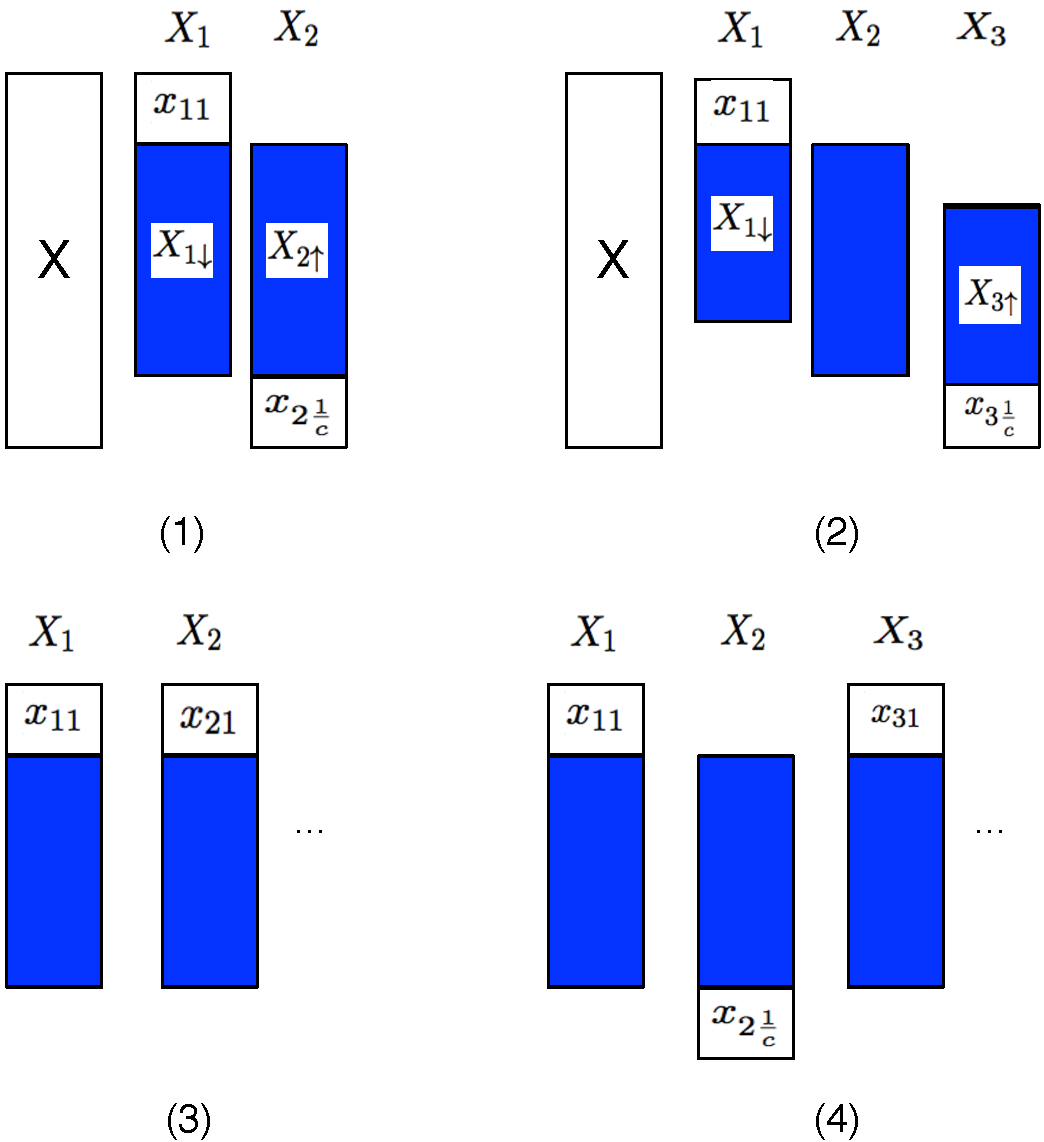
\includegraphics[width=4.8in]{fig/stream_database1.pdf}
\caption{\label{stream_db1} Blocks in blue are shared by more than one databases. Blocks in white are owned by only one database. (1) Composition of $F(X_{1})$ and $F(X_{2})$. It has ``good" independence since each $X_{i}$ owns one block. (2) Composition of queries on three streaming databases. Cannot leverage ``good" independence, because each block in $X_{2}$ is shared by two databases. (3) Composition of queries in the standard DP case. The blue blocks refer to the query while the white blocks refer to the independent noise. (4) It works as long as each streaming database owns one block of ``private" block.}
\end{figure}
\begin{figure}[th]
\centering
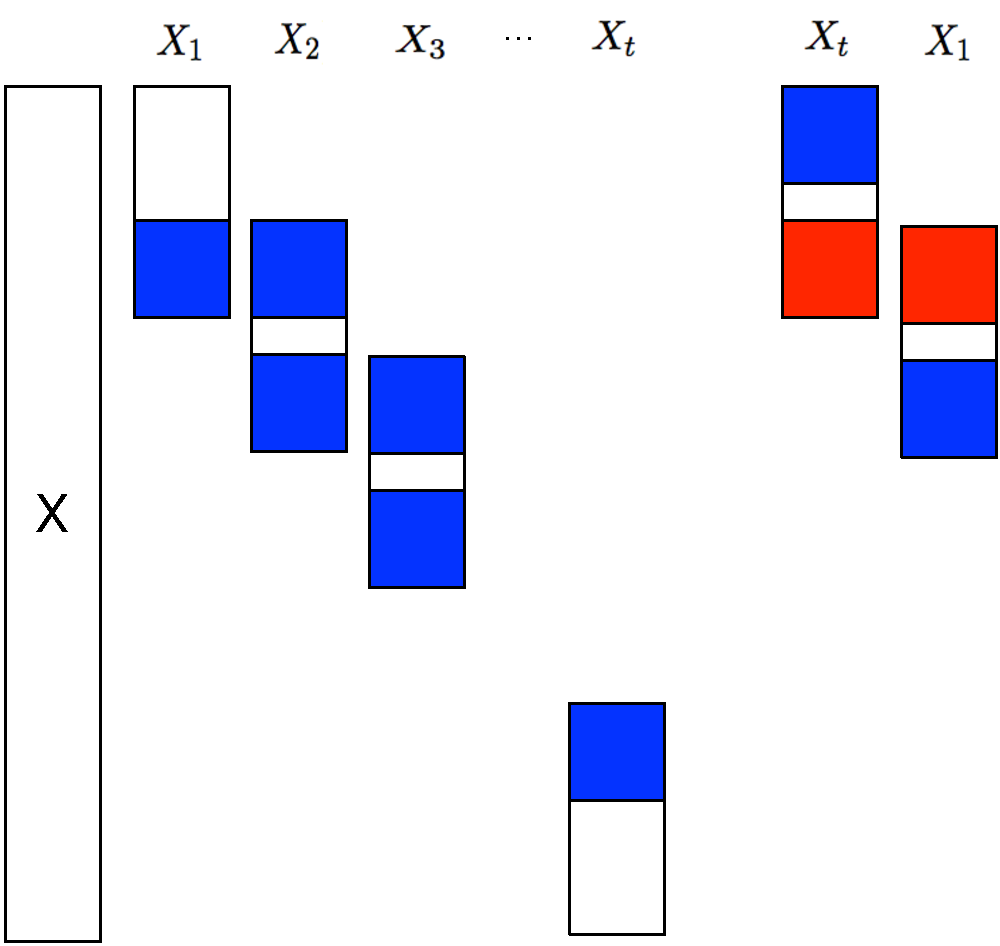
\includegraphics[width=4.8in]{fig/stream_database2.pdf}
\caption{\label{stream_db2} Blocks in blue are shared by more than one databases. Blocks in white are owned by only one database. Construct streaming databases such that each $X_{i}$ owns a block of $cn$ rows by itself. In this figure, the middle block is always private. At each time step, $\frac{1+c}{2} n$ rows need to be generated independently. We can connect $X_{t}$ back to $X_{1}$ to make the big database $X$ circular. Now, $X$ has size of  $\frac{1+c}{2} nt$}
\end{figure}

{\bf Problem setting} \\
Let $X$ be a database in the streaming setting. Let $X_{i}$ represent the portion of $X$ that is currently held at time step $i$. We assume that at each time step, a fraction of $c$ of the database is replaced. We assume the oldest rows are always the ones replaced, and that $X$ has row drown i.i.d. from some distribution $D$. Let $n$ be the size of each $X_{i}$. This means that the first $n$ rows of $X$ constitute $X_{1}$, rows $cn+1$ through $cn+n$ constitute $X_{2}$, and so forth. $X$ has size $n+cn(t-1)$, where $t$ is the total number of time steps being considered. $1/c$ is the total number of time steps a given row will be present for. See (1) and (2) in Figure~\ref{stream_db1}. 
\\
\\
{\bf Hypothesis}\\
We now consider a query $F: \, {\cal U}^{n} \rightarrow \mathbb{R}^{d}$ on each $X_{i}$. 
Let $D_{F}$ be the distribution that draws a database of size $n$, with each row chosen i.i.d. from $D$. Let $aux_{F}$ be $F$'s auxiliary information, which consists of any $(1-c)n$ rows of the database. Now, assume $F$ is $(\epsilon, \delta, \Delta_{F}, \Gamma)$-CW private with some simulator $sim_{F}$, where $\Delta$ chooses the database according to $D_{F}$ and the auxiliary information is $aux_{F}$ as stated above.

Let $G(X) = (F(X_{1}), F(X_{2}) , \dots, F(X_{t}))$ be the composite query that runs $F$ at each time step. We show $G$ is $(? \epsilon, ? \delta, \Delta, \Gamma)$ -CW private.
\\
\\
{\bf Notations }\\
For each $X_i$ of size $n$, we represent it by $1/c$ blocks (each has $cn$ rows). Namely, let $X_{i}=\xblock{i}$, where $x_{ij}$ denote the $j$th block in $X_{i}$. Let $\xdownk{i}{k} = [x_{i (k+1)}, x_{i (k+2)} , \dots, x_{i \frac{1}{c}}]^{\top}$ and $\xupk{i}{k} = [x_{i 1}, x_{i2} , \dots, x_{i (\frac{1}{c}-k)}]^{\top}$. We use $\xdown{i}$ to denote $\xdownk{i}{1}$ and $\xup{i}$ to denote $\xupk{i}{1}$. Notice that $\xdownk{i}{k} = \xupk{i+k}{k}$ (specifically $\xdown{i} = \xup{i+1}$), which are the shared blocks between $X_{i}$ and $X_{i+k}$. See (1) and (2) in Figure~\ref{stream_db1}.

Let $S=(S_{1}, S_{2}, \dots, S_{t} )$ be any set from $\mathbb {R} ^{d \times t}$, where $S_{j}$ is determined by the values of $(s_{1}, s_{2} , \dots, s_{j-1})$. Let $S_{-t}$ denote set $(S_{1}, S_{2}, \dots, S_{t-1} )$.
\\
\\
{\bf Proof for the base case}\\
The base case is when $G(X) = (F(X_{1}) , F(X_{2}))$. See (1) in Figure~\ref{stream_db1}.
For any set $S= (S_{1}, S_{2})$, we have
\[
\conpr{G(X) \in S}{ \priv = v }
\]
$\priv =v$ will be omitted from now on.
\[
=\conpr{F(X_{2}) \in S{2}}{ F(X_{1}) \in S_{1}} \cdot Pr[F(X_{1}) \in S_{1}]
\]
\begin{equation}
=(\Sigma_{s_{1} \in S_{1}} \conpr{F(X_{2}) \in S{2}}{  F(X_{1}) = s_{1}} \cdot Pr[F(X_{1}) = s_{1}])\cdot Pr[F(X_{1}) \in S_{1}]
\end{equation}
We focus on $\conpr{F(X_{2}) \in S{2}}{  F(X_{1}) = s_{1}} $.
\[
\conpr{F(X_{2}) \in S{2}}{  F(X_{1}) = s_{1}} = \Sigma_{z} \conpr{F(X_{2}) \in S{2}}{  F(X_{1}) = s_{1}, \xup{2} =z} \cdot Pr [\xup{2} = z]
\]
\[
= \Sigma_{z} \conpr{F(\xup{2}, \xbot{2}) \in S{2}}{ F(x_{11}, \xdown{1})=s_{1}, \xup{2}=z} \cdot Pr [\xup{2} = z]
\]
\[
= \Sigma_{z} \conpr{F(\xup{2}, \xbot{2}) \in S{2}}{ F(x_{11}, \xup{2})=s_{1}, \xup{2}=z} \cdot Pr [\xup{2} = z]
\]
Given $\xup{2}=z$ and $\xbot{2}$ and $x_{11}$ are i.i.d. generated, functions $F(\xup{2}, \xbot{2})$ and $F(x_{11}, \xup{2})$ are independent with each other. Only $S_{2}$ depends on the value $s_{1}$. By the assumption that $F$ is $\cwp{F}$-CW private with simulator $sim_{F}$, we have
\[
\leq \Sigma_{z} (e^{\epsilon}  \conpr{sim_{F}(\alt{2}) \in S{2}}{ F(X_{1})=s_{1}, \xup{2}=z}+\delta) \cdot Pr [\xup{2} = z]
\]
\[
=e^{\epsilon}  \conpr{sim_{F}(\alt{2}) \in S{2}}{ F(X_{1})=s_{1}}+\delta
\]
By equation (1), we have
\[
Pr [G(X) \in S] \leq e^{\epsilon}  Pr({sim_{F}(\alt{2}) \in S{2}}, { F(X_{1}) \in S_{1}})+\delta
\]
\begin{equation}
=e^{\epsilon} \conpr{ F(X_{1}) \in S_{1}} {{sim_{F}(\alt{2}) \in S{2}}} \cdot Pr [{sim_{F}(\alt{2}) \in S{2}}] +\delta
\end{equation}
Similarly, $
\conpr{ F(X_{1}) \in S_{1}} {sim_{F}(\alt{2}) \in S{2}}=
$
\begin{equation}
\Sigma_{s_{2}\in S_{2}} \conpr{ F(X_{1}) \in S_{1}} {sim_{F}(\alt{2}) = s_{2}} \cdot Pr [sim_{F}(\alt{2}) = s_{2}]
\end{equation}
We focus on $\conpr{ F(X_{1}) \in S_{1}} {sim_{F}(\alt{2}) = s_{2}}$, which equals to
\[
\Sigma_{z} \conpr{ F(X_{1}) \in S_{1}} {sim_{F}(\alt{2}) = s_{2}, \xdown{1} =z} \cdot Pr[\xdown{1}=z]
\]
\[
=\Sigma_{z} \conpr{ F(x_{11}, \xup{2}) \in S_{1}} {sim_{F}({\bf alt}(\xdown{1}, \xbot{2})) = s_{2}, \xdown{1} =z} \cdot Pr[\xdown{1}=z]
\]
Notice that $sim_{F}({\bf alt}\xdown{1}, \xbot{2}))$ can be seen a composite function $sim_{F} \circ {\bf alt}$ on $\xbot{2}$. Given $\xdown{1}=z$ and  that $\xbot{2}$ and $x_{11}$ are i.i.d. generated, functions $F(x_{11}, \xdown{1})$ and $sim_{F}({\bf alt}(\xdown{1}, \xbot{2}))$ are independent with each other. Only $S_{1}$ depends on the value $s_{2}$. By the assumption that $F$ is $\cwp{F}$-CW private with simulator $sim_{F}$, we have
\[
\leq (e^{\epsilon} \Sigma_{z} \conpr{ sim_{F}(X_{1}) \in S_{1}} {sim_{F}(\alt{2}) = s_{2},\xdown{1} =z}+\delta) \cdot Pr[\xdown{1}=z]
\]
\[
=e^{\epsilon} \conpr{ sim_{F}(X_{1}) \in S_{1}} {sim_{F}(\alt{2}) = s_{2}}+\delta
\]
By equation (2) and (3), we have
\begin{equation}
\conpr{ F(X_{1}) \in S_{1}} {sim_{F}(\alt{2}) \in S{2}} \leq e^{\epsilon} \conpr{ sim_{F}(X_{1}) \in S_{1}} {sim_{F}(\alt{2}) \in S_{2}}+\delta
\end{equation}
By equations (2) and (3), we have
\[
Pr[G(X) \in S] \leq e^{2\epsilon} Pr[sim_{F} (\alt{1}) \in S_{1} , sim_{F} (\alt{2}) \in S_{2}] + 2\delta \quad \blacksquare
\]
\\
\\
{\bf The problem when compose three queries}\\
In this case, $G(X) = (F(X_{1}) , F(X_{2}), F(X_{3}))$. See (2) in Figure~\ref{stream_db1}. 

For any set $S= (S_{1}, S_{2}, S_{3})$, we can easily derive a similar equation as (2) above
\begin{equation}
Pr [G(X) \in S] \leq e^{\epsilon}  Pr({sim_{F}(\alt{3}) \in S{3}}, { F(X_{2}) \in S_{2}}, { F(X_{1}) \in S_{1}})+\delta
\end{equation}
But it appears we {\bf cannot proceed} any further from here. It is hard to leverage a kind of independence between $X_{2}, X_{1}$ and $X_{3}, X_{2}$ simultaneously. This is because $X_{2}$ does not have a block that is independent with both $X_{1}$ and $X_{3}$; each row in $X_{2}$ is shared by either $X_{1}$ or $X_{3}$. For the general case when $t \geq 3$, databases in the middle could have the same problem. 
\\
\\
{\bf The condition to make the composition work}\\
Intuitively, when each $X_{i}$ has at least one ``private" block (not shared by any other $X_{j}$), the composition should work.
\begin{enumerate}
\item As we can see in (1) in Figure~\ref{stream_db1}, the base case (when compose only two queries) satisfy this condition. 
\item In the standard DP case, the mechanism is $F=f(X)$+noise, where $f$ is  the query and noise is independently generated at each time step. At each time step $i$, $F$ can be seen as a query on a larger database $X_{i} = X \cup x_{i1}$, where $x_{i1}$ corresponds to the database of the noise. Notice that $X$ remains the same while $x_{i1}$ is regenerated independently each time. In other words, each $X_{i}$ owns a private block of $x_{i1}$. See (3) in Figure~\ref{stream_db1}.
\end{enumerate}
\section{Streaming Setting 2}
{\bf Problem setting}\\
We use the same definitions and notations as before. Each $X_{i}$ has $n$ rows, or $1/c$ blocks. We construct each $X_{i}$ such that its middle block is private. At each time step, $\frac{(1+c)n}{2}$ rows need to be generated independently. For a total of t time steps, $X$ has size of $n+\frac{(1+c)(t-1)n}{2}$. See Figure~\ref{stream_db2}. 
\\
\\
{\bf Composition theorem}\\
Let $F$ be a query on each $X_{i}$. Assume $F$ is $\cwp{F}$-CW private with simulator $sim_{F}$, where $\Delta_{F}$ chooses the database according to some distribution and contains auxiliary information of any $(1-c)n$ rows of the database.

Let $G(X) = (F(X_{1}), F(X_{2}) , \dots, F(X_{t}))$ be the composite query that runs $F$ at each time step. Then, $G$ is $(t\epsilon, t \delta, \Delta, \Gamma)$ -CW private with simulator ${sim_{F}}^{t}$.
\\
\\
{\bf Extension}\\
\begin{enumerate}
\item The private block of each $X_{i}$ does not have to be in the middle. If so, the number of blocks that need to be generated at each step is different, though asymptotically remain the same. In other words, assume $F$ is $\cwp{F}$-CW private with a fraction of $r$ of the database as auxiliary information, an asymptotical fraction of $(1-r/2)$ rows need to be generated independently at each time step.
\item We can connect $X_{t}$ back to $X_{1}$ to make the big database $X$ circular. Then, $X$ has size of $\frac{1+c}{2}nt$. See Figure~\ref{stream_db2}. In the streaming setting, $X$ can be seen as the local database at the client end. The client has limited local memory, such that it has to replace the first streaming database $X_{1}$ after $t$ queries. 
\end{enumerate}

{\bf Extra Notations.} Let $\xmid{i}$ denote the set of blocks in $X_{i}$ but the middle one. Let $\xm{i}$ denote the middle block of $X_{i}$. In Figure~\ref{stream_db2},
$\xmid{i}$ contain the blues blocks while $\xm{i}$ is the white middle block in $X_{2} , \dots X_{t-1}$ .
\\
\\
{\bf Proof}\\
For any set $S=S_{1}, S_{2}, \dots , S_{t}$, we have
\begin{equation}
Pr[G_{t}(X) \in S] = \conpr{F(X_{t}) \in S_{t}}{ G_{t-1}(X) \in S_{-t}} \cdot Pr[ G_{t-1}(X) \in S_{-t}]
\end{equation}
We focus on $\conpr{F(X_{t}) \in S_{t}}{ G_{t-1}(X) \in S_{-t}}$, which equals to
\[
=\Sigma_{z} \conpr{F(X_{t}) \in S_{t}}{ G_{t-1}(X) \in S_{-t} , \xmid{t}=z}\cdot Pr[\xmid{t}=z]
\]
Given $\xmid{t}=z$, $F(X_{t})$ is a function on $\xm{t}$ and $G_{t-1}(X)$ is a function on blocks before $x_{t1}$. Since every block is generated independently, functions $F(X_{t})$ and $G_{t-1}(X)$ are independent with each other. Only $S_{t}$ depends on the value of $G_{t-1}(X)$. By the assumption that $F$ is $\cwp{F}$-CW private with simulator $sim_{F}$, we have
\[
\leq \Sigma_{z} (e^{\epsilon} \conpr{sim_{F} (\alt{t}) \in S_{t}}{G_{t-1}(X) \in S_{-t},  \xmid{t}=z} + \delta)\cdot Pr[\xmid{t}=z]
\]
\[
=e^{\epsilon} \conpr{sim_{F} (\alt{t}) \in S_{t}}{G_{t-1}(X) \in S_{-t}} + \delta
\]
Combined with equation (6), we have
\begin{equation}
Pr[G_{t}(X) \in S] \leq e^{\epsilon} Pr[ sim_{F} (\alt{t}) \in S_{t}, G_{t-1}(X) \in S_{-t}] + \delta
\end{equation}
Now, $Pr[ sim_{F} (\alt{t}) \in S_{t}, G_{t-1}(X) \in S_{-t}] $
\[
=\conpr{F(X_{t-1}) \in S_{t-1}}{sim_{F} (\alt{t}) \in S_{t}, G_{t-2}(X) \in S_{-(t-1)}}
\]
\begin{equation}
\cdot Pr[sim_{F} (\alt{t}) \in S_{t}, G_{t-2}(X) \in S_{-(t-1)}]
\end{equation}
We focus on $\conpr{F(X_{t-1}) \in S_{t-1}}{sim_{F} (\alt{t}) \in S_{t}, G_{t-2}(X) \in S_{-(t-1)}}$.
\[
=\Sigma_{z'} \conpr{F(X_{t-1}) \in S_{t-1}}{sim_{F} (\alt{t}) \in S_{t}, G_{t-2}(X) \in S_{-(t-1)}, \xmid{t-1}=z'}
\] 
\[
\cdot Pr [\xmid{t-1}=z']
\]
Given $\xmid{t-1}=z'$, $F(X_{t-1})$ is a function on $\xm{t-1}$, $sim_{F} (\alt{t})$ is a function on blocks after $\xbot{t-1}$ and $G_{t-2}(X)$ is a function on blocks before $x_{(t-1)1}$. Since every block is generated independently, functions $F(X_{t-1})$ is independent with both $sim_{F} (\alt{t})$ and $G_{t-2}(X)$. Only $S_{t-1}$ depends on the value of $G_{t-2}(X)$ and $sim_{F} (\alt{t})$. By the assumption that $F$ is $\cwp{F}$-CW private with simulator $sim_{F}$, we have
\[
\leq  \Sigma_{z'} (e^{\epsilon}\conpr{sim_{F}(\alt{t-1}) \in S_{t-1}}{sim_{F} (\alt{t}) \in S_{t}, G_{t-2}(X) \in S_{-(t-1)}, \xmid{t-1}=z'} +\delta)
\]
\[
\cdot Pr [\xmid{t-1}=z']
\]
\[
=e^{\epsilon}\conpr{sim_{F}(\alt{t-1}) \in S_{t-1}}{sim_{F} (\alt{t}) \in S_{t}, G_{t-2}(X) \in S_{-(t-1)}} +\delta
\]
Combined with equation (8), we have
\[
Pr[ sim_{F} (\alt{t}) \in S_{t}, G_{t-1}(X) \in S_{-t}]
\]
\begin{equation}
\leq e^{\epsilon}Pr[ {sim_{F} (\alt{t}) \in S_{t}, {sim_{F}(\alt{t-1}) \in S_{t-1}}, G_{t-2}(X) \in S_{-(t-1)}}] +\delta
\end{equation}
By equation (7) and equation (9), we have
\[
Pr[G_{t}(X) \in S] \leq e^{2\epsilon} Pr[ {sim_{F} (\alt{t}) \in S_{t}, {sim_{F}(\alt{t-1}) \in S_{t-1}}, G_{t-2}(X) \in S_{-(t-1)}}]+ 2\delta
\]
Repeat the same procedure on $F(t-2), \dots , F(1)$, we can show
\[
Pr[G_{t}(X) \in S] \leq e^{t\epsilon} Pr[ {sim_{F} (\alt{t}) \in S_{t}, \dots , {sim_{F}(\alt{1}) \in S_{1}}}]+ t\delta \quad \blacksquare
\]

\end{document}
